\documentclass[a4 paper]{article}
\usepackage[inner=2.0cm,outer=2.0cm,top=2.5cm,bottom=2.5cm]{geometry}
\usepackage{setspace}
\usepackage[rgb]{xcolor}
\usepackage{verbatim}
\usepackage{subcaption}
\usepackage{amsgen,amsmath,amstext,amsbsy,amsopn,tikz,amssymb}
\usepackage[colorlinks=true, urlcolor=blue,  linkcolor=blue, citecolor=blue]{hyperref}
\usepackage[colorinlistoftodos]{todonotes}
\usepackage{rotating}
\usepackage{booktabs}
\newcommand{\ra}[1]{\renewcommand{\arraystretch}{#1}}

\newtheorem{thm}{Theorem}[section]
\newtheorem{prop}[thm]{Proposition}
\newtheorem{lem}[thm]{Lemma}
\newtheorem{cor}[thm]{Corollary}
\newtheorem{defn}[thm]{Definition}
\newtheorem{rem}[thm]{Remark}
\numberwithin{equation}{section}

\newcommand{\homework}[6]{
   \pagestyle{myheadings}
   \thispagestyle{plain}
   \newpage
   \setcounter{page}{1}
   \noindent
   \begin{center}
   \framebox{
      \vbox{\vspace{2mm}
    \hbox to 6.28in { {\bf CSE 211:~Discrete Mathematics \hfill {\small (#2)}} }
       \vspace{6mm}
       \hbox to 6.28in { {\Large \hfill #1  \hfill} }
       \vspace{6mm}
       \hbox to 6.28in { {\it Instructor: {\rm #3} \hfill Name: {\rm #5} \hfill Student Id: {\rm #6}} \hfill}
       \hbox to 6.28in { {\it Assistant: #4  \hfill #6}}
      \vspace{2mm}}
   }
   \end{center}
   \markboth{#5 -- #1}{#5 -- #1}
   \vspace*{4mm}
}

\newcommand{\problem}[2]{~\\\fbox{\textbf{Problem #1}}\hfill (#2 points)\newline\newline}
\newcommand{\subproblem}[1]{~\newline\textbf{(#1)}}
\newcommand{\D}{\mathcal{D}}
\newcommand{\Hy}{\mathcal{H}}
\newcommand{\VS}{\textrm{VS}}
\newcommand{\solution}{~\newline\textbf{\textit{(Solution)}} }

\newcommand{\bbF}{\mathbb{F}}
\newcommand{\bbX}{\mathbb{X}}
\newcommand{\bI}{\mathbf{I}}
\newcommand{\bX}{\mathbf{X}}
\newcommand{\bY}{\mathbf{Y}}
\newcommand{\bepsilon}{\boldsymbol{\epsilon}}
\newcommand{\balpha}{\boldsymbol{\alpha}}
\newcommand{\bbeta}{\boldsymbol{\beta}}
\newcommand{\0}{\mathbf{0}}


\begin{document}
\homework{Homework \#4}{Due: 17/01/21}{Dr. Zafeirakis Zafeirakopoulos}{Gizem S\"ung\"u}{}{}
\textbf{Course Policy}: Read all the instructions below carefully before you start working on the assignment, and before you make a submission.
\begin{itemize}
  \item It is not a group homework. Do not share your answers to anyone in any circumstance. Any cheating means at least -100 for both sides. 
  \item Do not take any information from Internet.
  \item No late homework will be accepted. 
  \item For any questions about the homework, send an email to gizemsungu@gtu.edu.tr
  \item The homeworks (both latex and pdf files in a zip file) will be
  submitted into the course page of Moodle.
  \item The latex, pdf and zip files of the homeworks should be saved as
  "Name\_Surname\_StudentId".$\{$tex, pdf, zip$\}$.
  \item If the answers of the homeworks have only calculations without any formula or any explanation -when needed- will get zero.
  \item Writing the homeworks on Latex is strongly suggested. However, hand-written paper is still accepted $\textbf{IFF}$ hand writing of the student is clear and understandable to read, and the paper is well-organized. Otherwise, the assistant cannot grade the student's homework.
\end{itemize}

\problem{1}{15+15=30}
Consider the nonhomogeneous linear recurrence relation $a_n$ = 3$a_{n-1}$ + $2^n$ .\\
\subproblem{a} Show that whether $a_n$ = $-2^{n+1}$ is a solution of the given recurrence relation or not. Show your work step by step.\newline
Yes and it's shown
\solution
\newline
\subproblem{b} Find the solution with $a_0$ = 1.
\solution
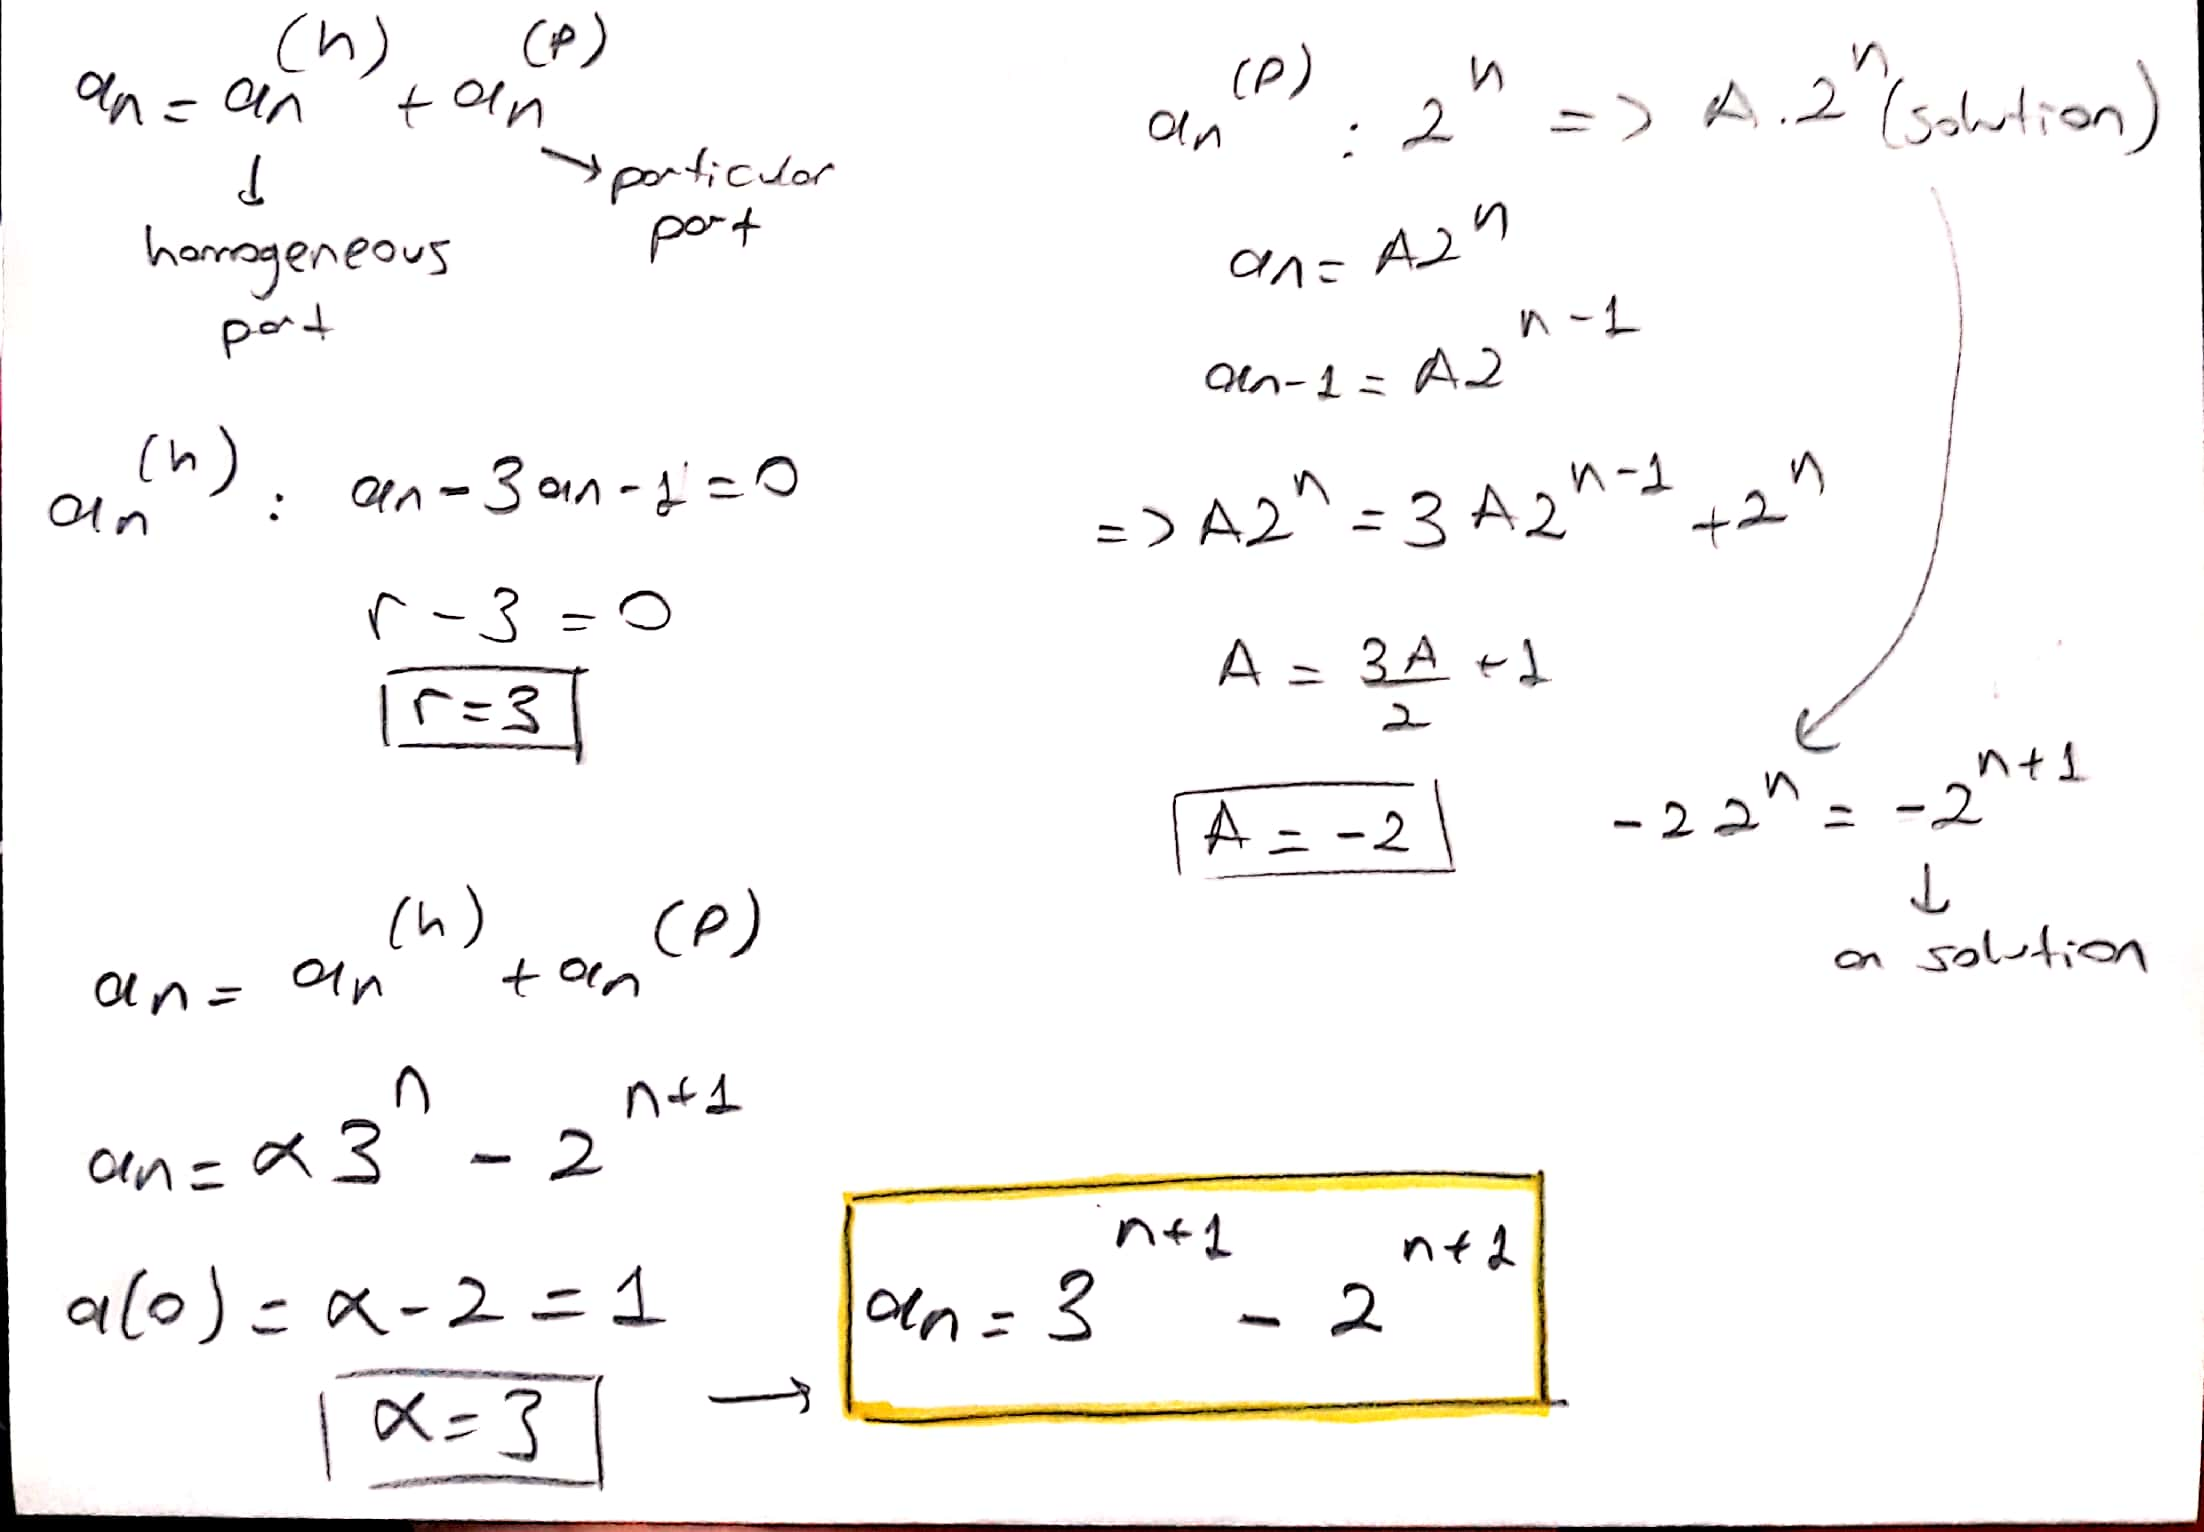
\includegraphics[scale=0.2]{1}
\newline



\problem{2}{35}
Solve the recurrence relation f(n) = 4f(n-1) - 4f(n-2) + $n^2$ for f(0) = 2 and f(1) = 5. 
\solution
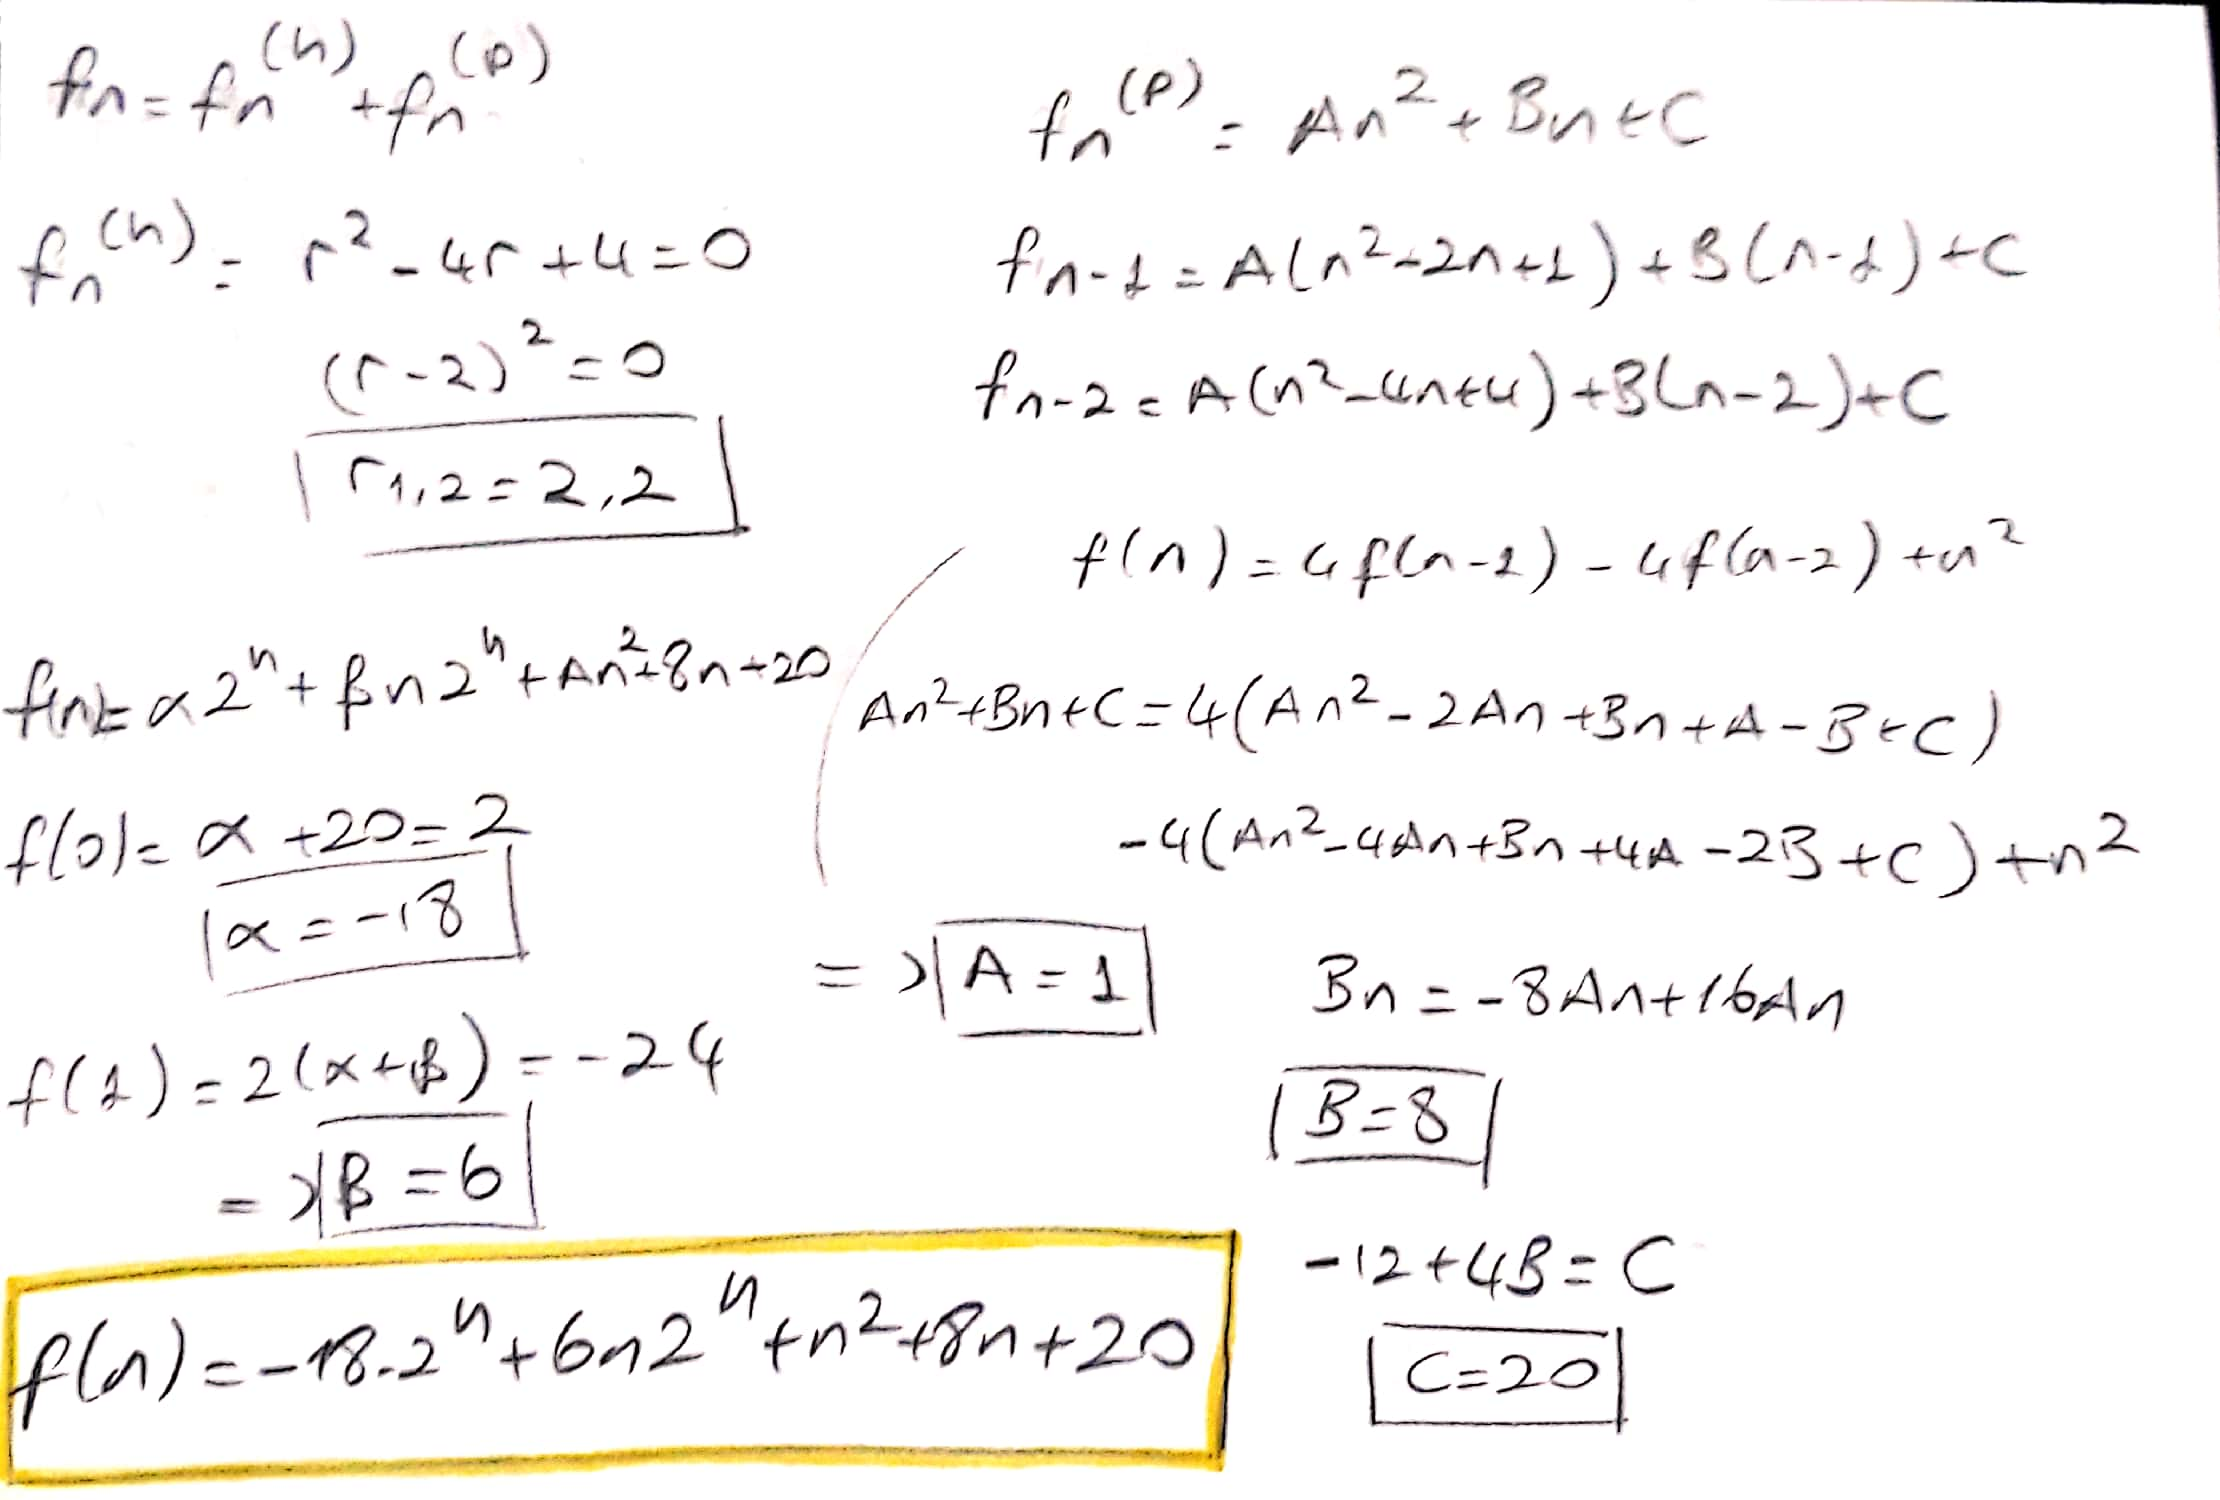
\includegraphics[scale=0.2]{2}
\newline



\problem{3}{20+15 = 35}
Consider the linear homogeneous recurrence relation $a_n$ = 2$a_{n-1}$ - 2$a_{n-2}$.
\subproblem{a} Find the characteristic roots of the recurrence relation.
\solution
\newline
\subproblem{b} Find the solution of the recurrence relation with $a_0$ = 1 and $a_1$ = 2.
\solution

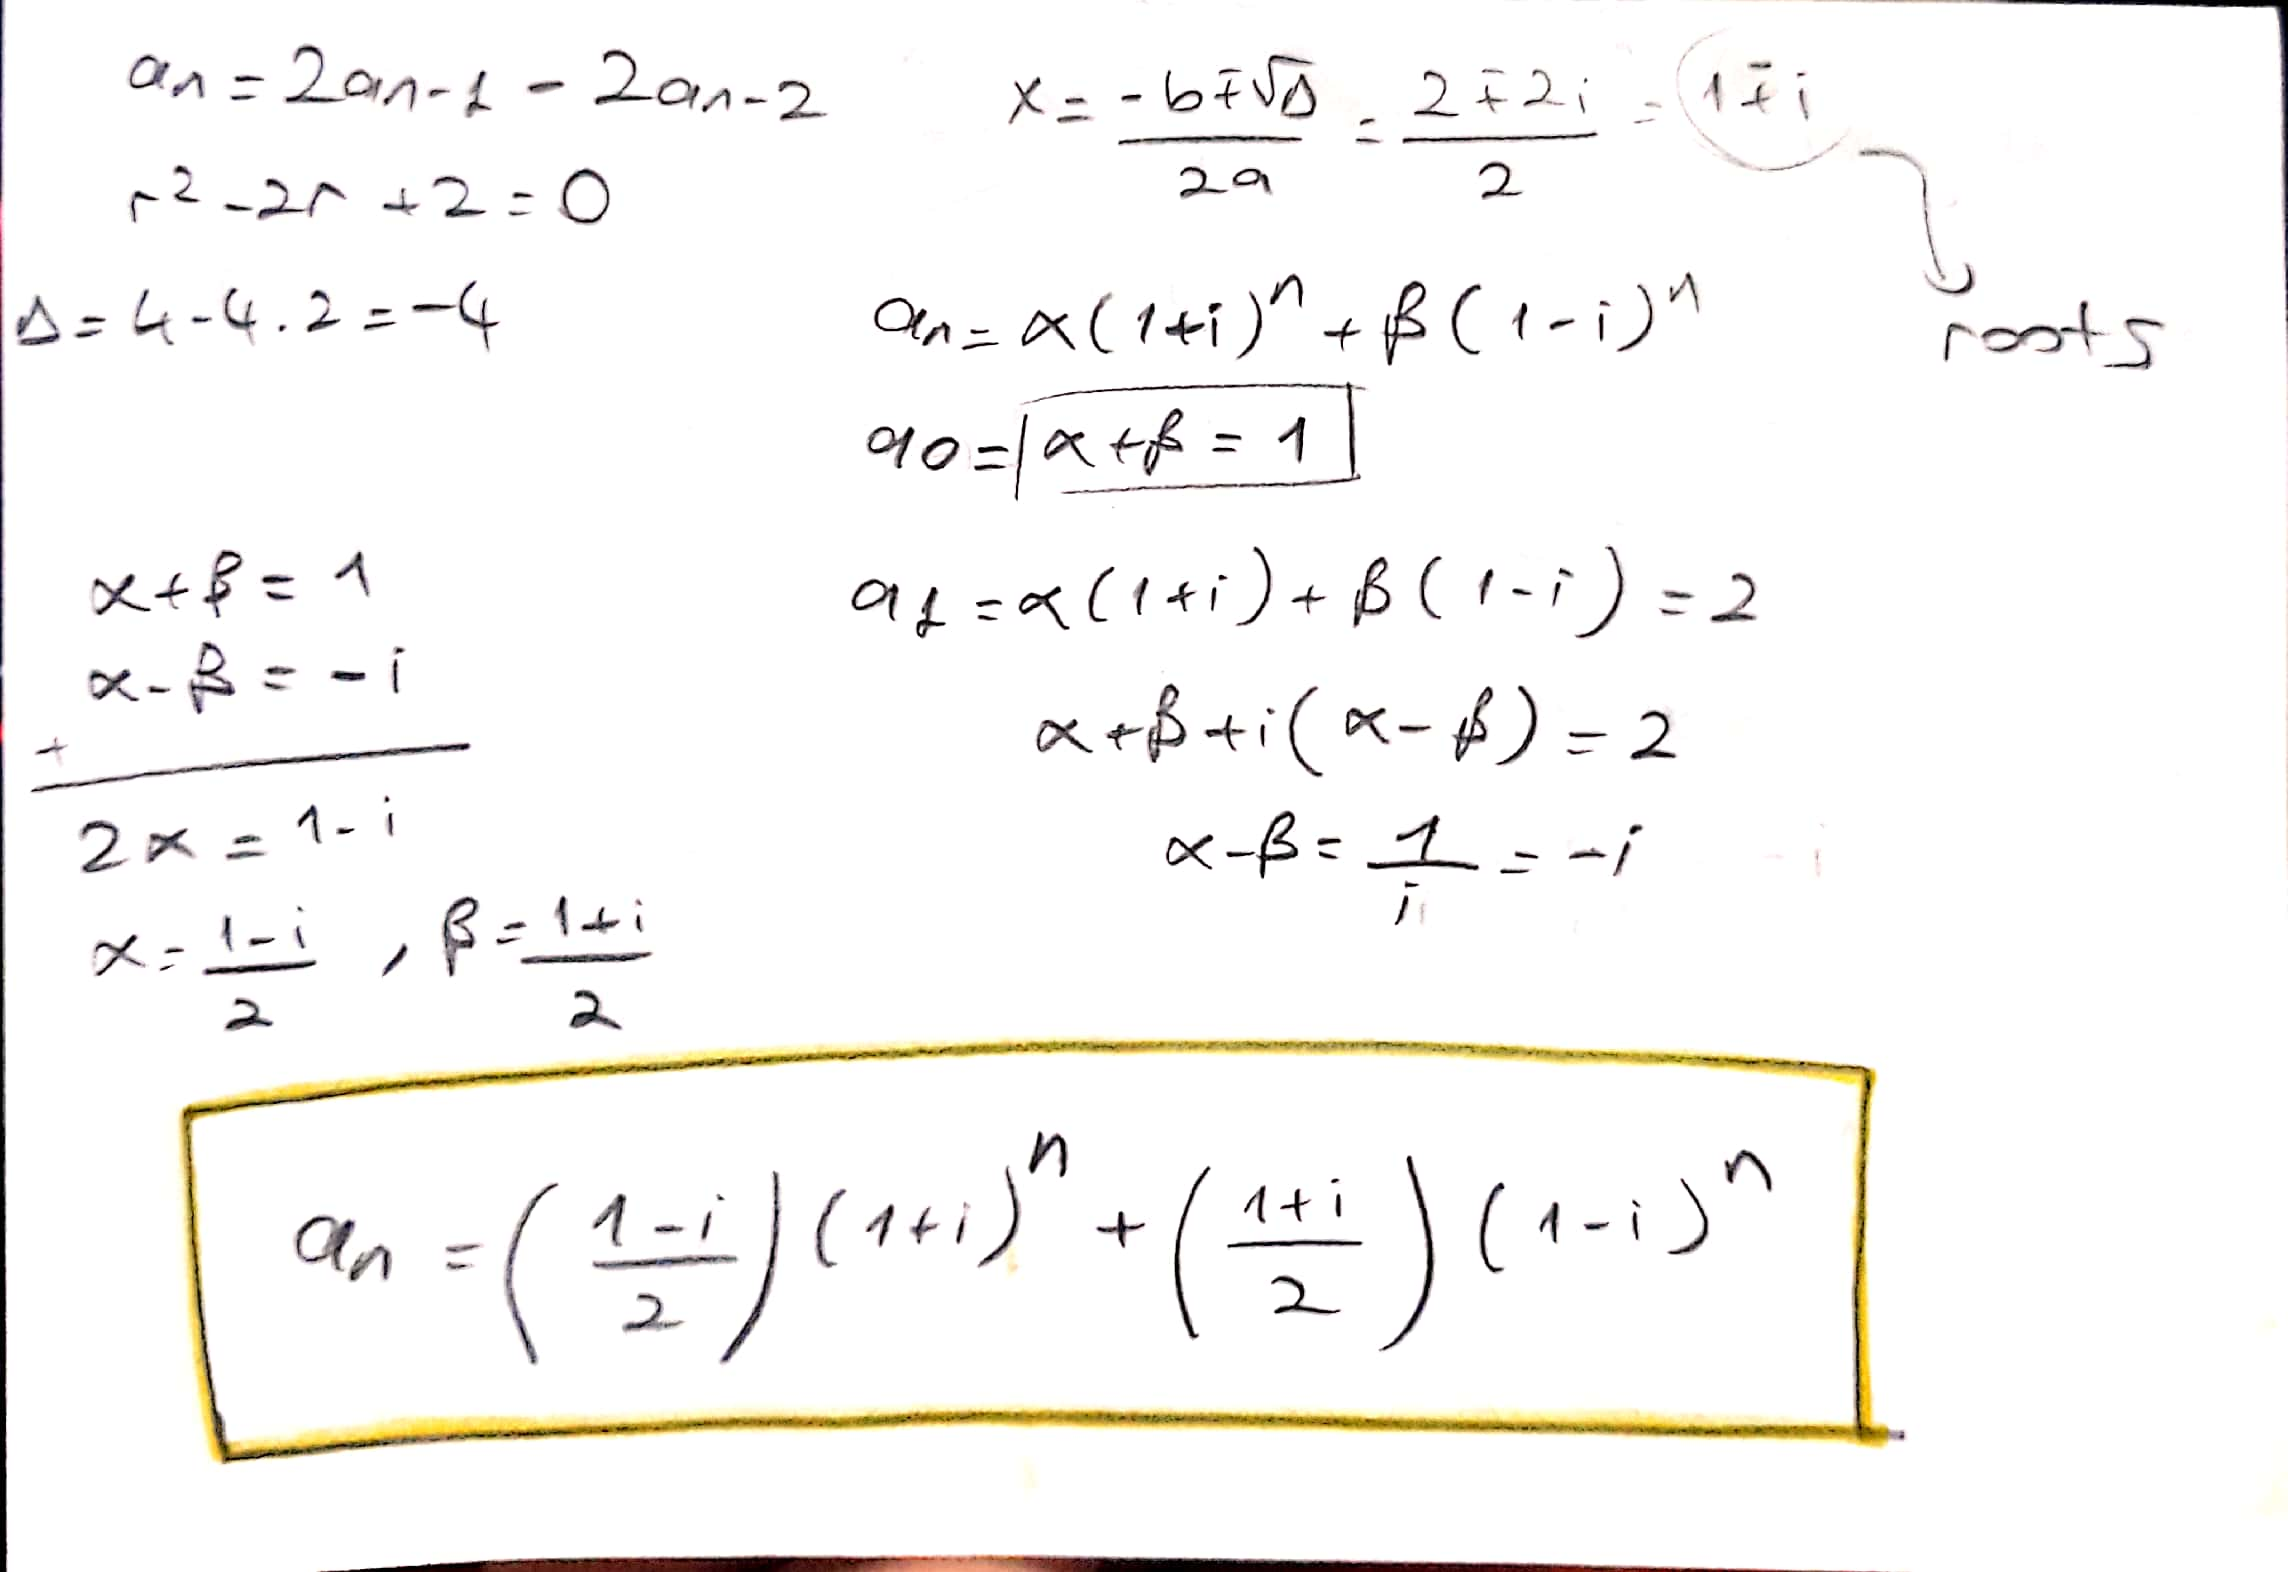
\includegraphics[scale=0.2]{3}


\end{document} 


